\documentclass{jdrp}

\bibliography{songes-de-l-uhumele/references} 

\newcommand*{\crg}{{\aurebesh\Large \$}} % Symbol for Galactic Credits

\hypersetup{
	pdftitle={SWR - Songes de l’Uhumele},
	pdfsubject={Scénario, Songes de l’Uhumele},
	pdfauthor={Marthym},
	pdfkeywords={starwars,savage,worlds,jdr,scenario},
	pdfcopyright={This work is licensed under the Creative Commons Attribution-ShareAlike 4.0 International License.}
}

\begin{document}

	\begin{titlepage}

	\begin{center}
		\hspace*{\vfill}
		\noindent\Huge\jedifont{Star Wars Redemption}\\ 
		\noindent\fontsize{50}{70}\jedifont{\$}
		\noindent\fontsize{50}{70}\jedifont{\#}\\
		\noindent\fontsize{40}{60}\jedifont{Songes de l’uhumele}
		\hspace*{\vfill}
	\end{center}

	%\hspace*{\vfill}

	\noindent\makebox[\textwidth]{
		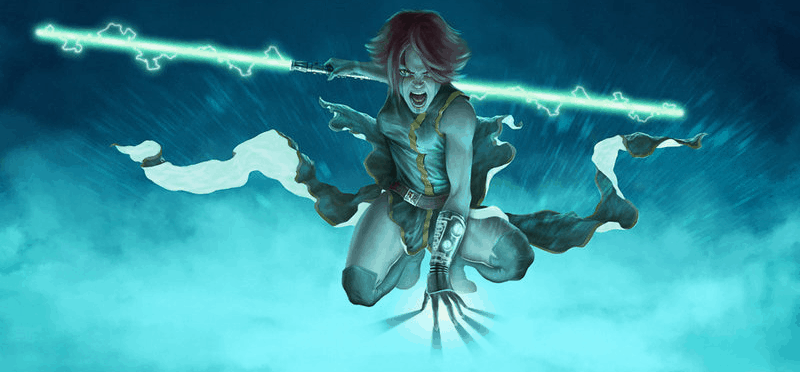
\includegraphics[width=\paperwidth]{_img/cover-bg.png}}
	\begin{tikzpicture}[overlay]
		\node[minimum width=200pt,minimum height=200pt] at (15,11){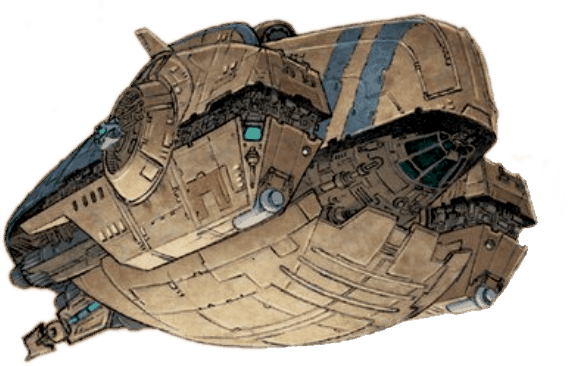
\includegraphics[width=240pt]{_img/songes-de-l-uhumele/uhumele.png}};
	\end{tikzpicture}}
	\end{titlepage}

	\onecolumn
	\section{Contexte du Scénario}
		\begin{wrapfigure}{R}{180pt}
			\centering
			
\includegraphics[width=180pt]{_img/songes-de-l-uhumele/bomo-greenbark.png}
			\caption{\label{fig:bomo-greenbark}Bomo Greenbark}
		\end{wrapfigure}

	Voici un court scénario sur le thème de \nameref{sec:uhumele}. Ce scénario bien qu’indépendant est fortement lié à la campagne "Dos au Muur" de \citetitle{jdrp-starwars}. C’est un scénario écrit pour faire patienter entre deux étapes de la campagne (2 et 3). 

	L’idée est que l’un des personnages, sensible à la force et possédant \textit{Sens de Force} a une vision d’un évènement passé. En l’occurrence, la tentative de sauvetage de Resa, la fille de \textbf{Bomo Greenbark} par l'équipage de l’Uhumele. Les joueurs jouent alors le rôle des membres de l’équipage (avec leur propre fiche de perso). Ce système à l’intérêt d’introduire l’Uhumele dans la campagne Dos au Muur mais aussi de ne pas modifier les circonstances entre les 2 scénarios. Pas besoin de faire des raccords tirés par les cheveux.

	Bien-sûr, ce scénario peut aussi être joué hors du contexte de la campagne Dos au Muur, en remplaçant l’introduction “vision” par, par exemple, une introduction à base de contrat.

	A noter que ce scénario est plutôt fait pour des héros notre ou orienté gentils.

	Ce scénario se passe normalement en -19 pendant les derniers affrontements entre l’armée des clones et les armées de droïde de la Confédération des Systèmes Indépendants.

	\twocolumn

	\section{introduction}
	L’équipage de \nameref{sec:uhumele} quitte Nouvelle Plympto au lendemain d’une grande bataille qui a obligé les habitants à évacuer pour se mettre à l’abri. \'A cette époque, l’équipage du Uhumele venait de mettre la main sur une cargaison inconnue et dangereuse qui les pousse à éviter l’Empire au maximum. C’est pourquoi quand l’Empire est arrivé pour s’opposer aux droïdes, le vaisseau a quitté la planète en urgence. Mais dans la précipitation, la famille de \textbf{Bomo Greenbark} n’a pas eu le temps d’embarquer dans l’Uhumele et s’est trouvée évacuée par l’Empire.

	Quand Bomo se renseigne pour savoir sur quel vaisseau a été évacué sa famille, il apprend que sa femme et sa fille ont embarqué sur le \textbf{Sevarog} un vaisseau à destination d’Orvax IV, plate-forme galactique majeure du trafic d’esclaves. Le scénario commence au moment où Bomo demande de l’aide à l’équipage de l’Uhumele pour récupérer sa fille.

	\section{orvax iv}
	Plate-forme galactique majeure du trafic d’esclaves, Orvax IV est situé dans la bordure extérieure et peuplé d’à peu près toutes les espèces que compte la galaxie. L’Empire comme la République ne s’y sont jamais intéressé et laisse cette planète faire ses affaires comme elle le souhaite.

	La planète se présente comme un vaste marché aux esclaves, trié en catégorie, races, age, genre, \ldots.

	Première étape, retrouver le \textbf{Sevarog} à bord duquel est arrivée la famille de Bomo. N’importe qui au spatioport donnera le numéro du quai où se trouve le vaisseau. Bien sur, les esclaves ont été débarqués et la famille de Bomo ne se trouve plus à bord. S’il l'interroge, le capitaine du Sevarog apprend que les esclaves déportés par l’Empire sont stockés dans une fosse au nord du spatioport en dessous de la boutique “U2”.

	\section{Fosse u2}
	En tant qu’entrepôt de stockage de l’Empire, la zone est sous bonne garde, des \nameref{sec:storm-trooper}s patrouilles régulièrement dans le coin et l’arrière de la boutique est gardé.

	Les héros ont le choix de passer par les égouts, de négocier ou de passer en force, a vous de doser la difficulté en fonction de leur niveau.

	Une fois arrivé dans le sous-sol de la boutique, les héros trouvent plusieurs fosses, grillagé sur le dessus, où s’entassent des centaines d’esclaves, majoritairement des femmes et des filles qui implorent pour qu’on les libère.

	Si les héros appellent Mesa ou Resa (la femme et la fille de Bomo), une des esclaves dans une fosse sur la droite sort la main de la grille et dit~:

	\begin{quotebox}
    	Ici, ici, venez, je connais Mesa et Resa.

    	Faite moi sortir de là et je vous dirais où se trouve Mesa et Resa.
	\end{quotebox}
	Aux héros de voir comment ils gèrent ça. S’ils sont rentrés en mode discrétion et qu’ils ressortent avec un ou plusieurs esclaves les jets de \textit{Discrétion} prennent un malus de \textbf{-2}. S’ils font sortir tous les esclaves, la \textit{Discrétion} n’est plus possible.

	Une fois que l’esclave se sent en sûreté, elle leur explique que Resa a été vendu et que Mesa a été tuée en voulant s’interposer. Bomo est bouleversé et ses camarades doivent le retenir pour qu’il ne s’en prenne pas à l’esclave. Cette dernière se souvient du nom de l’acheteur, \textbf{Dezono Qua}, ce dernier a dit qu’il l’emmenait sur \textbf{Esseles}.

	\section{La forteresse d’Esseles}
	\textbf{Dezono Qua} est un humain excentrique et riche qui vit dans une forteresse miniature en haut d’une colline sur \textbf{Esseles}. Les autorités locales sont au courant que ses affaires ne sont pas toutes blanche, mais sa fortune le tient à l’abri des lois locales. Il vit seul dans sa forteresse protégée par une armée de droïdes.\\ 

	Le but ici est de retrouver \textbf{Dezono Qua} ou \textbf{Resa} et d’opérer une extraction en bonne et due forme. Lancer d10+d4 pour savoir ou se trouve Dezono Qua. Les pièces sont numérotées sur la carte de 1 à 14~:
	\begin{enumerate}
		\item Salle à manger (Dining Room)
		\item Cuisine (Kitchen)
		\item Entrepôt (Storage)
		\item Quartier des dommestiques (Servant Quarter)
		\item Salon (Lounge)
		\item Petit salon (Nook)
		\item Bibliothèque (Library)
		\item Réserve (Supply Room)
		\item Petit bureau (Nook)
		\item Salle de détente principale (Main Divining Room)
		\item Salle de détente secondaire (Sub Divining Room)
		\item Salon personnel (Personnal Room)
		\item Chambre (Sleep Chamber)
		\item Chambre Secrète (Secret Room)
	\end{enumerate}
	\onecolumn
	\subsection{Forteresse d’Esseles}\label{sec:forteresse-esseles}
	\begin{figure}[!h]
		\centering	
		\begin{tikzpicture}[overlay, anchor=north]
			\node[rotate=90] at (-10,-11.5) {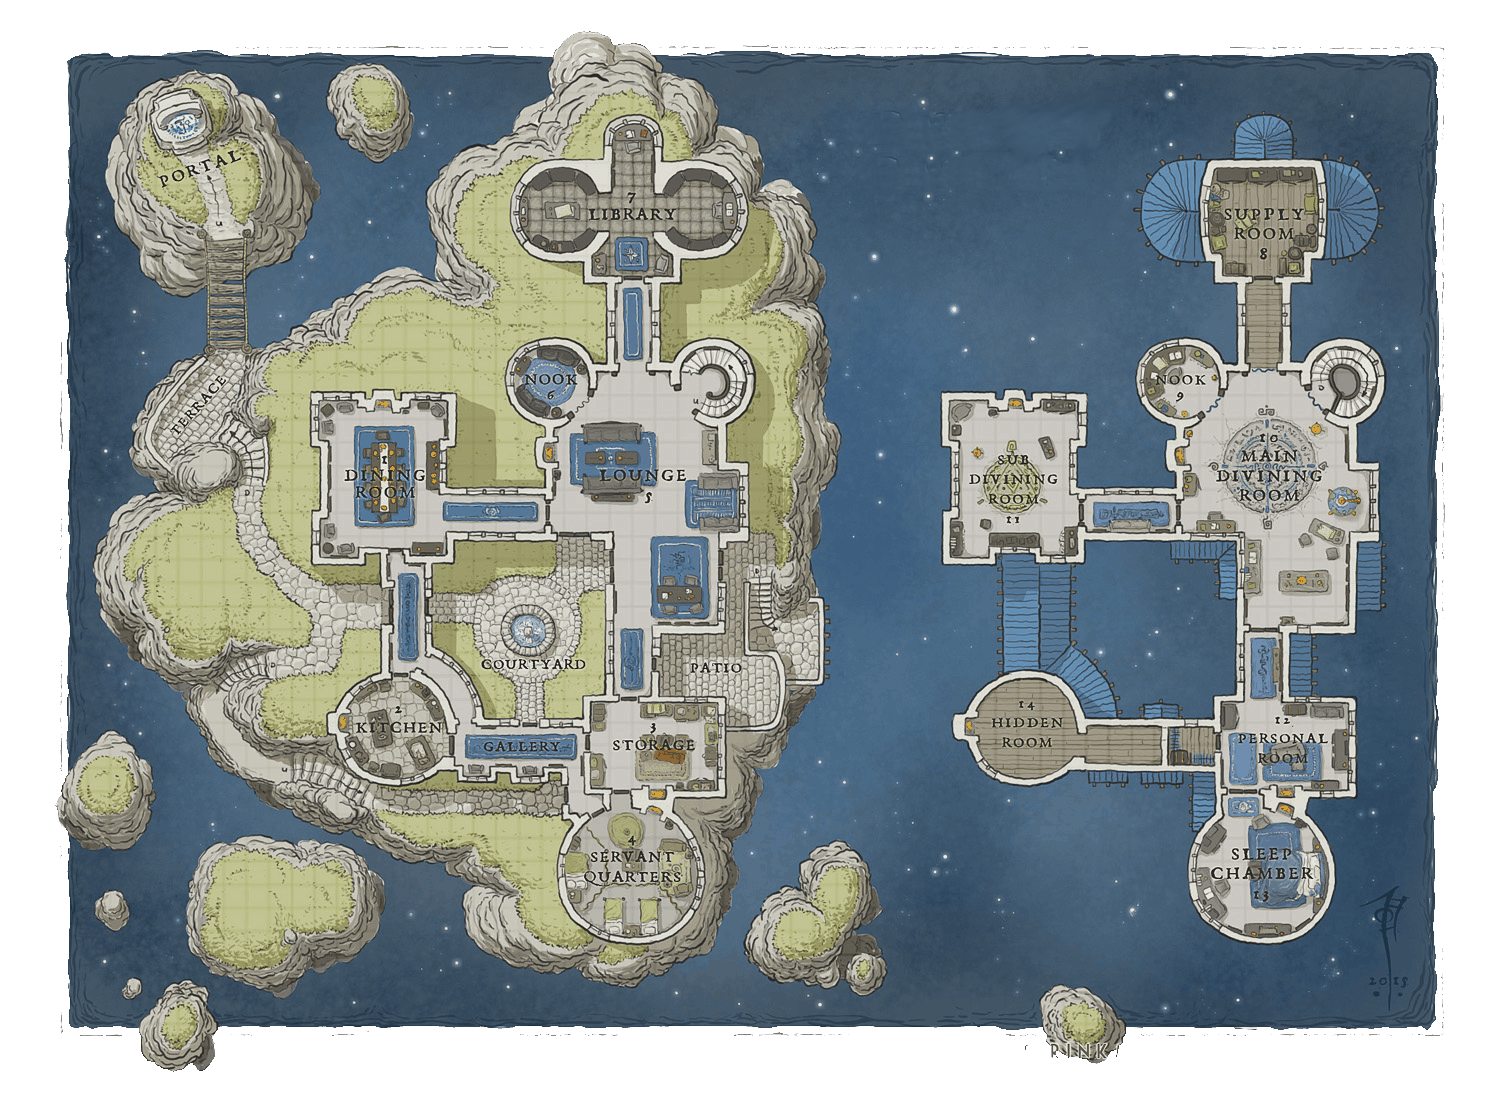
\includegraphics[width=1.05\textheight]{_img/songes-de-l-uhumele/forteresse-esseles.png}};
		\end{tikzpicture}
	\end{figure}
	\twocolumn

	\begin{paperbox}{Notes sur la carte}
	N'étant pas un artiste dans l’âme j’ai pris la carte sur internet. Donc à la base c’était pas la forteresse de Dezono Qua mais les pièces collent pas mal avec le scénario. En dehors des «~Divining Room~» que j’ai remplacé par «~Salle de détente~».

	Attention, les joueurs ne sont pas sensé voir la carte, surtout la pièce secrète~!

	\cite{sirinkman-deviantart}.
	\end{paperbox}

	On ne jette pas de dés pour Resa, car les héros ne peuvent pas la trouver (même s’ils peuvent la chercher). 

	Ici aussi les joueurs ont le choix de rentrer en force ou en mode infiltration. \'A vous de doser la difficulté en fonction de vos joueurs. L’armée de \textbf{Dezono Qua} est composé de \nameref{sec:droide-b1} et de \nameref{sec:droideka}. Dezono possède aussi un \nameref{sec:droide-protocole} qui reste avec lui en permanence.

	Si les héros choisissent de rentrer en force, toutes les pièces de la forteresse se verrouillent et devront être \textit{Piraté} ou \textit{Forcé}.\\

	\ldots baston time \ldots \\

	\subsection{Dezono Qua}
	\'A la fin, vos joueurs trouvent Dezono Qua. Un petit bonhomme trapu et bien en chair. Ce dernier ne semble pas traumatisé plus que ça par l’intrusion d’inconnus dans sa demeure.

	\begin{quotebox}
    	Bien le bonjour messieurs ! Que me vaut cette visite impromptue~?

    	\textit{\ldots bla bla les héros vous racontent bla bla \ldots}

    	Je vois très bien de qui vous parlez, la jeune Nosaurienne. Une enfant délicieuse, au sens propre du terme \ldots
	\end{quotebox}

	Si les héros n'ont pas compris, Dezono a mangé Resa, pour de vrai. En effet, certain milliardaire excentrique avaient ce genre de pratique, manger des extratérestres !

	Sous le coup de l’émotion \textbf{Bomo} saute sur Dezono et comment à le rouer de coups encore et encore, même après que le milliardaire ne soit mort, il n’arrive plus à s’arrêter~!

	Une fois retourné au Uhumele, Bomo rase la forteresse avant de quitter la planète.

	\section{Epilogue}
	C’est ici que s’arrête le scénario. Pour ce qui est de l’XP, le scénario était classique et pas trop long, \textbf{2XP} semble une bonne récompense.


	\newpage
	\section{Annexes}
	\subsection{l’Uhumele}\label{sec:uhumele}
	\noindent
\includegraphics[width=\textwidth]{_img/songes-de-l-uhumele/uhumele-pano.png}

	L'Uhumele est un vaisseau cargo de classe inconnue, actif notamment pendant et après la Guerre des Clones. Son capitaine est le Yarkora Schurk-Heren. On ignore quand et dans quelles conditions Schurk-Heren devint capitaine de l’Uhumele et comment son équipage le rejoignit. Ce qui est sûr, c'est qu’il a de bonnes raisons de détester la République et de craindre l’Empire qui lui succède.

	L’Uhumele est avant tout un vaisseau de contrebande, comme un bon nombre de cargos en apparence en règle. De ce fait, il est doté d’un armement susceptible de pouvoir le sortir des situations délicates dans lesquelles il se fourre. L’une de ces armes est un bras rétractable situé sous le ventre de l’appareil, au bout duquel se trouve une petite tourelle blaster, ressemblant à celle des Canonnières clones. Bien que cette tourelle permette d’avoir un très vaste angle de tir, elle rend la situation du tireur précaire car très exposé. 

	\hspace{12em}
	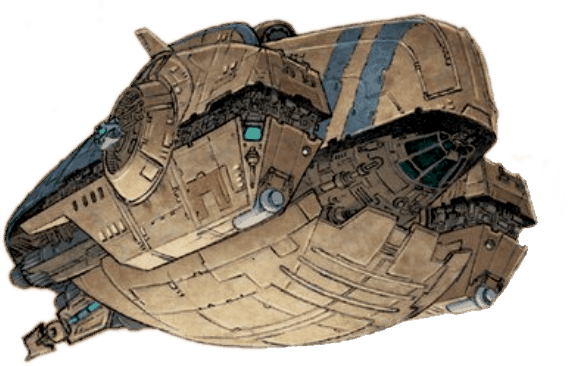
\includegraphics[width=0.8\textwidth]{_img/songes-de-l-uhumele/uhumele.png}
	\section{Bestiaire}

\subsection{Storm Trooper} \label{sec:storm-trooper}
\begin{figure}[h!]
    \centering
    
\includegraphics[height=200pt]{_img/dos-au-muur/stormtrooper.png}
\end{figure}
\paragraph{Background}
Soldats dévoué de l’empire. Certain sont des clones restant de la guerre des clones d’autres non. Ils sont entrainés au combat, équipé d’une bonne armure et armé de Fusil Blaster efficaces.

\paragraph{Traits}

\begin{itemtable}[ c c c c c ]
    \textbf{Agi} & \textbf{Int} & \textbf{\^Ame} & \textbf{For} & \textbf{Vig} \\
    d4           & d6           & d4             & d8           & d8
\end{itemtable}
\begin{itemtable}[ l X ]
    \textbf{Allure}      & 6 \\
    \textbf{Compétences} & Combat d10, Tir d10
\end{itemtable}

\paragraph{Défense}
\begin{itemtable}[ c c ]
    \textbf{Parade}     & \textbf{Résistance} \\
    7                   & 6 (+4)
\end{itemtable}

\paragraph{Attaque}
\begin{itemtable}[ X c c ]
    ~              & \textbf{Combat}   & \textbf{Dégats} \\
    Fusil Blaster  & -                 & 2d8 (3)
\end{itemtable}


\newpage


	\onecolumn
	\nocite{*}
	\printbibliography
\end{document}